\chapter{Preparation}

This project inherently covers many different areas, as it aims to use methods of programming languages to solve problems of array programming practitioners (e.g. in machine learning). In this chapter:
\begin{itemize}
    \item We begin with a description of the array programming model in the context of Python (Section \ref{array-programming-model}).
    \item We then consider the pointful array paradigm and its inspirations in Section \ref{pointful-array-programming}.
    \item Section \ref{domain-specific-languages} looks into the topic of embedding domain-specific languages.
    \item We introduce classic functional programming (Section \ref{functional-programming-patterns}) and compiler techniques (Section \ref{compiler-techniques}).
    \item Lastly, I give a project requirements analysis (Section \ref{requirements-analysis}) and starting point (Section \ref{starting-point}).
\end{itemize}

\section{Array programming model}
\label{array-programming-model}

Much of today's deep learning and scientific computing workflows takes place in the \textit{array programming model} of \textcite{iverson1962programming}. 
This style is dominated by \textbf{whole-array operations}. 
The leading Python library for efficiently processing multidimensional arrays, NumPy, is no exception \cite{harris2020array}. 
NumPy focuses on CPU execution and is implemented in highly-optimised C, playing a central role in numeric programming across the entire Python ecosystem. 
NumPy's design is motivated by Python's significant runtime overheads -- it is profitable to offload to large units of work. The core data structure is the \texttt{\textbf{ndarray}} -- a multidimensional rectangular array of primitive values (e.g. floats). We shall just call these \textit{arrays}. 
% Some sources use the name \textit{tensors}.

Many modern Python array libraries are based on NumPy, including ubiquitous deep learning frameworks like PyTorch, TensorFlow, and JAX \cite{frostig2018compiling, paszke2019pytorch, abadi2016tensorflow}, which take advantage of hardware accelerators. This similarity is seen as a merit, though many inconsistencies cause problems with interoperability \cite{meurer2023python}.

We now introduce common terms when dealing with arrays. The number of dimensions of an array is called its \textit{rank}. We call arrays of rank 0  -- scalars, rank 1 -- vectors, and rank 2 -- matrices. Rectangular arrays have a consistent size in every dimension (\textit{axis}), and as such have a \textit{shape}, which is a tuple of natural numbers the same length as the rank. Indexing into an array $a$ of shape $(d_0, ... d_{k-1}) \in \mathbb{N}^k$ is defined for exactly the indices $(i_0, ..., i_{k-1}) \in \mathbb{N}^k$ such that $0 \le i_p < d_p$, and is usually denoted $a[i_0, ..., i_{k-1}]$. Axes are indexed from 0, and here we say that $i_p$ indexes into axis $p$.
\begin{figure}[h]
    \centering
    $$ A = \begin{bmatrix}
        1 & 2 & 3 \\ 
        4 & 5 & 6
    \end{bmatrix} \text{ is a rectangular array, but } B = \begin{bmatrix}
    0 & 1 & \\
    0 & 1 & 2
    \end{bmatrix} \text{ is not.} $$
    $$ \mathrm{shape}(A) = (2, 3)  \quad \mathrm{rank}(A) = 2 \quad A[0, 2] = 3 $$
    \caption{Examples of array concepts}
    \label{fig:array-examples}
\end{figure}

\subsection{Programming in NumPy} 

We now give a summary of the key features of NumPy. Efficiency of many of the following primitives relies on the use of \textbf{strides} in the \texttt{ndarray} representation \cite{harris2020array} -- we treat this as an implementation detail. For clarity throughout this section, functions corresponding to NumPy primitives are written in \texttt{monospace}.

\paragraph{Broadcasting}

The obvious kind of whole-array operation is an \textbf{elementwise operator}:
$$ \begin{bmatrix} 1 & 2 \\ 3 & 4 \end{bmatrix} 
+ \begin{bmatrix}1 & -1 \\ -1 & 1 \end{bmatrix}
= \begin{bmatrix}1 + 1 & 2 - 1 \\ 3 - 1 & 4 + 1 \end{bmatrix}
= \begin{bmatrix}2 & 1 \\ 2 & 5 \end{bmatrix} $$
\textit{Pointfully}, we define the action $C = A + B$ on matrices as $C[i, j] = A[i, j] + B[i, j]$ for all valid $i, j$. The relevant primitive is \texttt{numpy.add}. 
% Elementwise operations assert operands are of the same shape.

But what about the cases where arrays do not have matching shapes? Consider scaling a matrix, i.e. $L = \lambda A$, defined $L[i, j] = \lambda \cdot A[i, j]$. \textbf{Broadcasting} generalises elementwise operations to the case where only a subset of axes is present in each array. NumPy approaches this by \textit{repeating axes of size 1}, unambiguously indexed with $0$. For instance, consider the outer product $C = a \otimes b$ ($C[i, j] = a[i] \cdot b[j] $). To compute it NumPy, we shape $a$ and $b$ as a row vector and column vector respectively, i.e. $\mathrm{shape}(a) = (n, 1)$ and $\mathrm{shape}(b) = (1, m)$. Then:
$$ C = \texttt{multiply}(a, b) \iff C[i, j] = a[i, {\color{blue} j}] \cdot b[{\color{blue} i}, j] = a[i, 0] \cdot b[0, j] $$
% Thanks to broadcasting, we avoid copying the data caused by repeating the arrays along an axis explicitly. 
This can be concise and elegant, but the main drawback is that broadcasting is ad-hoc and difficult to formalise. The condition for matching up axes of size $d$ and $d'$ is $d = d' \lor d = 1 \lor d' = 1 $. Disjunctions are widely known to be difficult to handle in e.g. type inference.
Not only that, but without compile-time information on shapes involved, there are $2^{\mathrm{rank}}$ possible computational behaviours of a broadcast.

\paragraph{Shape manipulation} But how do we obtain arrays in a form suitable for computing the required operation with broadcasting? NumPy offers various primitives that efficiently change the shape of an array without copying its data (thanks to using strides). Say that in the above example $a$ and $b$ were just vectors. Then we may use \texttt{numpy.expand\_dims} with the axis index to add:
\begin{align*}
&\mathrm{shape}(a) = (n) \implies \mathrm{shape}(\texttt{expand\_dims}(a, \texttt{axis=1})) = (n, 1) \\
&C = a \otimes b = \texttt{multiply} \left( \texttt{expand\_dims}(a, \texttt{axis=1}), \texttt{expand\_dims}(b, \texttt{axis=0}) \right)
\end{align*}
It is worth noting that the inverse of \texttt{expand\_dims} (a.k.a. \texttt{unsqueeze}) is \texttt{squeeze}. Now consider $C = A + A^T$ ($C[i, j] = A[i, j] + A[j, i]$). NumPy offers the \texttt{numpy.transpose} primitive, which permutes axes:
\begin{align*}
&A^T = \texttt{transpose}(A, (1, 0)) \iff A^T[i, j] = A[j, i] \\
&C = A + A^T = \texttt{add}(A, A^T) = \texttt{add}(A, \texttt{transpose}(A, (1, 0))) 
\end{align*}
All of these primitives generalise to multiple dimensions. 
The main source of problems are the axis indices and permutations, which get harder to reason about as we generalise to more and more dimensions. 

\needspace{3em}
\paragraph{Reductions}
Operations we have considered so far cannot \textit{accumulate} data. Though the paradigm does not forbid simply looping in Python, the faster idiomatic approach is a \textit{reduction}. To compute a so-called tropical matrix product,\footnote{The tropical $(\min, +)$ algebra is useful in various shortest path problems on graphs.} we use \texttt{numpy.min}, parametrised by the index of the axis to reduce over:
\begin{align*}
&C[i, j] = \min_k A[i, k] + B[k, j] \\
&C = \texttt{min} \left( \texttt{add} \left(\texttt{expand\_dims}(A, \texttt{axis=1}), \texttt{expand\_dims}(A, \texttt{axis=0}) \right), \texttt{axis=1} \right)
\end{align*}

\paragraph{Generality} NumPy could be called a \textbf{first-order} interface, since its primitives cannot be parametrised with functions. Thus, we can only broadcast and reduce with some operations. This leads to limitations of what can be expressed efficiently. If not for \texttt{numpy.argmax}, one would be forced to use a slow Python loop:
\begin{center}
\begin{cminted}{python}
p = 0
for i in range(len(a)): 
    if a[i] > a[p]: p = i
\end{cminted}
\end{center}
Though there exist more efficient implementations of the above routine, they are necessarily slower than a native (e.g. C++) implementation due to Python's dynamic typing.
% This is due to the overheads caused by using a Python loop.
% It is worth noting that a framework like JAX does expose custom reductions.

\subsection{Jagged arrays}

\textit{Jagged} (non-rectangular) arrays are used less often than their counterpart. 
They cause irregular parallelism, which is more difficult to implement efficiently. 
NumPy and similar frameworks forbid them entirely. This is not unprecedented -- the same constraint is present in the Futhark array language \cite{henriksen2017futhark}, and preservation of rectangular arrays can be seen as one of the core features of the dependent type system in Dex. We shall also consider jagged arrays to be an error.

\subsection{Types}

Python supports a form of gradual typing through optional \textit{type hints} (\textit{annotations}), written \mintinline{python}{name: type}. For instance, a function that takes an integer \texttt{x} and a string \texttt{t} and returns a string has the signature:
\begin{center}
\begin{cminted}{python}
(x: int, t: str) -> str
\end{cminted}
\end{center}
One can (and should) take advantage of this system to document the behaviour of functions and allow some static analysis and type checking. This is facilitated via third party tools, such as \texttt{mypy}.

Unfortunately, static typing is notoriously difficult in the array programming model \cite{liu2020type}. In general, keeping track of array sizes already invites dependent types \cite{henriksen2021towards}. Consider typing for array element types and ranks. There are many problems that such a type system faces in NumPy, but primarily:
\begin{itemize}
    \item An extremely broad API surface, with no underlying theoretical principles, with arrays often constructed arbitrarily based on passed arguments.
    \item Complex dependencies between types. For instance, broadcasting of arrays of ranks $k$ and $\ell$ produces a rank $\max(k, \ell)$. Similarly, un/squeezing 1-dimensions increments/decrements the rank. Type-level arithmetic like this is generally difficult to encode.
    \item Even element types are difficult to model, as they are often dependent on arguments (e.g. \texttt{dtype}) to NumPy routines. Otherwise, they follow C-like type promotion, which also complicates inference.
\end{itemize}

\section{Pointful array programming}
\label{pointful-array-programming}

In functional programming, one can distinguish \textbf{pointful} and \textbf{point-free} (tacit, or ``pointless'') styles -- see examples in Figure \ref{fig:point-haskell}. This distinction essentially considers whether data flow is given by variable names, or driven with combinators. A classic example is that of $\lambda$ and SKI calculi, which are respectively pointful and point-free. Both have the same expressive power, but it is known that compiling $\lambda$ to SKI \textit{(bracket abstraction)} incurs an overhead, which is dependent on the expressiveness of the combinators \cite{lachowski2018complexity}. 
In essence, one can view the main result of this work as \textbf{bracket abstraction for array programs}.

\begin{figure}
\centering
\begin{subfigure}{.3\textwidth}
  \centering
    \begin{cminted}{haskell}
sum = foldr (+) 0
    \end{cminted}
      \caption{Point-free}
\end{subfigure}%
\begin{subfigure}{.3\textwidth}
  \centering
  \begin{cminted}{haskell}
sum [] = 0
sum (x:xs) = x + sum xs
  \end{cminted}
  \caption{Pointful}
\end{subfigure}
\caption{Point-free and pointful styles of a Haskell \texttt{sum} function}
\label{fig:point-haskell}
\end{figure}

We draw a similar distinction in array programming (following \textcite{paszke2021getting}).
The array programming model is said to be \textit{point-free}, because we reason about operations on whole arrays at a time, and not individual elements. 
In contrast, in \textit{pointful} (or \textit{index-oriented}) array programming it is central to think about arrays as functions, with each element defined in terms of its index. 
The pointful style pushes indexing operations to the forefront, and brings us closer to \textbf{mathematical notation} -- as per Iverson. We give a comparison between the \textit{point-free} NumPy and \textit{pointful} Dex in Figure \ref{fig:point-arrays}.

\begin{figure}
\centering
\begin{subfigure}{.4\textwidth}
  \centering
    \begin{cminted}{python}
c = multiply(
  transpose(a, (1, 0)),
  expand_dims(b, 1))
    \end{cminted}
      \caption{Point-free NumPy}
\end{subfigure}%
\begin{subfigure}{.4\textwidth}
  \centering
  \begin{cminted}{haskell}

c = for i j. a.j.i * b.j
  
  \end{cminted}
  \caption{Pointful Dex}
\end{subfigure}
\caption{Point-free and pointful array programs in NumPy and Dex}
\label{fig:point-arrays}
\end{figure}


\subsection{Einstein summation}

The need for a better notation for multidimensional operations became evident in the Python community, which looked towards \textbf{Einstein summation} as a solution. It is a notation used in physics for expressing linear algebra in an index-oriented fashion. In brief, indices which are repeated are implicitly summed over, and all indices span over the full size of the indexed axis \cite{aahlander2002einstein}. A matrix product $C = AB$ is written:
$$ C_{i,k} = A_{i,j} B_{j,k} $$
Einstein notation was the main influence on the \texttt{numpy.einsum} function, where the above is computed by \mintinline{python}{einsum("ij,jk->ik", a, b)}. This idea was expanded on by Tensor Comprehensions \cite{vasilache2018tensor}, and more recently in \texttt{einops} \cite{rogozhnikov2021einops}, which allows index-oriented shape manipulations, e.g.:
$$
\text{\mintinline{python}{einops.rearrange(x, "b h w c -> b c h w ()")}} \leadsto 
\text{\mintinline{python}{expand_dims(transpose(x, (0, 3, 1, 2)), 4)}}
$$
% CUT: Non-Python projects with similar inspiration include Taco \cite{kjolstad2017tensor} and the Tullio macro in Julia.


\subsection{Languages}

Dex is the most relevant example of a \textbf{pointful array language}, with its initial paper \cite{paszke2021getting} introducing the \textit{pointful/point-free} distinction. 
It features a value-dependent type system for keeping track of array sizes, embracing parallels between arrays and functions. 
However, its dependent type system would be impractical when embedded in Python, and it relies on a bespoke LLVM compiler.
% Its shortcomings are the bespoke LLVM compiler and need for binding code when used with other frameworks, both of which introduce friction in practical use. 
% It was not used as a basis for this project, as I found its type system to be too impractical in an embedded language.

One of the influences for Dex was $\tilde F$, introduced by \textcite{shaikhha2019efficient}. 
$\tilde F$ is used as a basis in a series of adjacent papers for researching array programming techniques.
In this project it influenced my own pointful array calculus.
However, $\tilde F$ does not have an open implementation, and its proposed compiler relies on C code generation, so this project takes a different approach to compilation. 

The array comprehensions of Single-Assignment~C can be seen as a precursor feature of pointful array programming \cite{scholz1994single}. Pointful DSLs often feature comprehension-like constructs, which are prevalent in modern programming languages generally (e.g. Python and Haskell). 
% CUT: Lastly, the Tensor Algebra Compiler (TACO) also features various (limited) pointful features. However, its Python interface is unwieldy, it mostly focuses on sparse linear algebra, and lacks interoperability with existing solutions.

% \subsection{Mapping to hardware}

% \subsection{Other approaches}

% \subsubsection{Functional}

% \subsubsection{Named tensors}

% \subsubsection{Macro-based}

\section{Domain-specific languages}
\label{domain-specific-languages}

The practice of creating domain-specific languages (DSLs) has a long history \cite{hudak1996building}. They are motivated by the observation that general capabilities like I/O, error handling, or even properties such as Turing-completeness are not always necessary language features. We can instead design languages specific to a given goal. Careful design choices simplify compilation and improve the programming experience.

\subsection{Embeddings}

A domain-specific language can be standalone, in which case it functions as an independent language with limited capabilities. 
However, a refined approach is \textbf{embedding} a DSL in a host language. 
In this project we focus on \textit{deep-embedded}\footnote{We further distinguish \textit{shallow embeddings}, which do not build up an intermediate representation of the program \cite{gibbons2014folding} and hence cannot undergo whole-program optimisations. One can see PyTorch as an example. The project proposal confused deep and shallow embeddings, but it was clear from context a JAX-style deep embedding was intended.} DSLs that work on the basis of term constructors -- they build up expressions in the DSL, and later execute them. 
In the context of Python, some DSLs directly inspect the program's AST instead of executing the code (compared in Figure \ref{fig:embeddings}). 
This style is inferior, as it is less predictable and cannot make good use of Python's features. 

\begin{figure}
\centering
\begin{subfigure}{.4\textwidth}
  \centering
  \begin{cminted}{python}
def foo(x, y):
  return JAX.lax.cond(
    x > 0, 
    lambda y: y+1, 
    lambda y: y-1, 
    y
  )
  \end{cminted}
  \caption{Deep-embedded DSL (JAX). The code is executed with tracing. The \texttt{cond} function is used, as \mintinline{python}{if} normally only works for Python \mintinline{python}{bool}s.}
\end{subfigure} \quad %
\begin{subfigure}{.4\textwidth}
  \centering
    \begin{cminted}{python}

@function
def foo(x, y):
  if x > 0: z = y+1
  else:     z = y-1
  return z

    \end{cminted}
      \caption{AST-based embedded DSL (TensorFlow). Python code is not executed, the \mintinline{python}{@function} decorator calculates a dataflow graph instead.}
\end{subfigure}
\caption{Domain-specific language embedding}
\label{fig:embeddings}
\end{figure}

Generally, deeply embedded DSLs are much easier to integrate with existing codebases and features of the host language.
In such DSLs \textbf{programs are values}, and hence the programmer can apply metaprogramming techniques to transform them \cite{atkey2009unembedding}. 
A special case of an embedding is a \textit{stringly-typed} DSL, where programs are expressed in strings which are parsed at runtime. An example in the scope of this work is the aforementioned \texttt{einops} library.  Similarly, one could see many regular expression interfaces as stringly-typed. The problematic reality of such embeddings is that they are difficult to generalise beyond a small core.

\subsubsection{Tracing} \label{tracing}

In the context of Python, a common approach to creating deep-embedded DSLs is \textbf{tracing}. It has found use in the JAX framework \cite{frostig2018compiling}. A DSL program is enclosed by a function in the host language, and to compile a program the function is \textit{traced} by calling it with placeholder (symbolic) arguments, representing the variable inputs. Computations are performed \textit{lazily} on these arguments -- no work is done immediately, and instead a computational graph is constructed. Once the function returns, the graph is captured and the program can be compiled and executed. An example is given in Figure \ref{fig:tracing}.

This approach leads to a kind of multi-stage programming, wherein before the results are determined, the entire program can first be collected and compiled. Tracing is often combined with techniques such as operator overloading, so that traced programs are written if they were \textit{eager}. A limitation of this approach is that runtime-dependent control flow (e.g. \mintinline{python}{if}, \mintinline{python}{while}) cannot be traced directly.
% as languages lack support for overloading \mintinline{python}{if} and \mintinline{python}{while} where the condition is not a known boolean value.
% (in this case, it would be a traced computation instead).


\begin{figure}
    \centering
    \begin{cminted}{python}
def f(x, y):
    x2 = x * x
    return x2 + y
assert (f(Var('x'), Var('y')) 
        == Add(Mul(Var('x'), Var('x')), Var('y')))
    \end{cminted}
    \caption{An annotated tracing example. \texttt{Var}, \texttt{Add}, and \texttt{Mul} are term constructors.}
    \label{fig:tracing}
\end{figure}

\section{Functional programming patterns}
\label{functional-programming-patterns}

\subsection{Applicative functors}

\textcite{mcbride2008applicative} introduced the notion of an \textit{applicative functor} -- a functional programming pattern that generalises monads and specialises functors. It is a well-behaved structure that defines certain primitive operations that behave well under composition. It is formed by a \textit{type constructor} $f$, meaning that for any type $\alpha$ there is some type $f\,\alpha$.

One of the central structures introduced in this work (the Axial) is shown to be an applicative, and so we introduce these operations here. We say a $f$ is an applicative functor if the following operations are defined:
\begin{align*}
\circledast &: f\,(\alpha \to \beta) \to f\,\alpha \to f\,\beta \\
\mathrm{return} &: \alpha \to f\,\alpha
\end{align*}
These operations must follow the \textit{applicative laws}, the exact formulation of which is out of scope. However, they can be seen in the light of \textit{homomorphisms} in a categorical sense, or just a notion of niceness under function composition. A definition upholding these laws shows the structure is in some way \textit{natural}. 

In this work we use a slight variation of $\circledast$ (which is pronounced \textit{apply}), called $\mathrm{lift}$:
\begin{align*}
\mathrm{lift}& : (\alpha \to \beta \to \gamma) \to (f\,\alpha \to f\,\beta \to f\,\gamma) \\ 
\mathrm{lift}&\,f\,a\,b = (f \circledast a) \circledast b
\end{align*}
One further generalises $\mathrm{lift}$ to arbitrary arities $\mathrm{lift}_k$ via an analogous construction (the above $\mathrm{lift}$ is $\mathrm{lift}_2$, and the base case $\mathrm{lift}_1$ is a $\mathrm{Functor}$ map). There exist a bijection between constructions of $\mathrm{lift}_2$ and $\circledast$.

Applicatives can be seen as an embellishment of values that permits application of similarly embellished transformations. Two examples of applicatives -- $\mathrm{List}$ and $\mathrm{ZipList}$ -- are shown in Figure \ref{fig:applicatives}.
%
\begin{figure}
\centering
\begin{subfigure}{.5\textwidth}
  \centering
  \begin{align*}
\mathrm{return}\,x &= [x] \\
\mathrm{lift}\,f\,a &= \mathrm{map}\,(\lambda\,(h, x) \ldotp h\,x)\,(f \times a)
  \end{align*}
  \caption{$\mathrm{List}$ (nondeterminism) applicative for arbitrary lists \\ -- pairwise application ($\times$ is the Cartesian product for lists)}
\end{subfigure}%
\begin{subfigure}{.5\textwidth}
  \centering
  \begin{align*}
\mathrm{return}\,x &= \mathrm{replicate}\,n\,x \\
\mathrm{lift}\,f\,a &= \mathrm{map}\,(\lambda\,(h, x) \ldotp h\,x)\,(\mathrm{zip}\,f\,a)
  \end{align*}
  \caption{$\mathrm{ZipList}$ applicative on lists of fixed length $n$ \\ -- respective application}
\end{subfigure}
\caption{Examples of applicative functors}
\label{fig:applicatives}
\end{figure}

\textit{Representable (Naperian) functors} are structures stronger than Applicatives, which generalise indexed collections. They are also useful abstraction in array programming \textcite{gibbons2016aplicative} and we follow their formulation to derive the Axial applicative.
% However, the structure we describe later on (the Axials) does not fully fit into this pattern, so we do not go into detail about them.

% \subsection{Monoids}

% A \textbf{monoid} is an algebraic structure defined through an associative operation $\oplus$ (concatenation) and identity element $\varepsilon$, i.e.:
% $$ (a \oplus b) \oplus c = a \oplus (b \oplus c) \quad a \oplus \varepsilon = \varepsilon \oplus a = a $$
% Monoids are an extremely important abstraction in parallel programming particularly thanks to the associativity property, thanks to which computation of \textit{reductions} can be efficiently parallelised via various work partitioning patterns. A simple divide-and-conquer halving pattern could be written as:
% $$ \bigoplus_{i=1}^{2n} f(i) = \bigoplus_{i=1}^{n} f(i) \oplus \bigoplus_{i=n+1}^{2n} f(i) $$

\section{Compilers}
\label{compiler-techniques}

Classically, a compiler consists of a lexer/parser (frontend), an assortment of analyses and tranformations (middle-end), and finally a code generator (backend), potentially with a runtime. In this project, the structure is slightly different. The frontend does not need a lexer/parser, as programs are constructed programmatically via the DSL embedding. We discuss what program representations are convenient for this purpose (Section \ref{representations}), and relevant compiler optimisations (Section \ref{general-optimisations}).

\subsection{Program representations} \label{representations}

A typical representation for programs is an \textbf{abstract syntax tree} (AST). 
Every node represents a single construct as a term in the program, and child nodes are its direct subterms. 
Since the structure is a tree, every node has exactly one parent -- except the root, which represents the entire program. 
In contrast, in a \textbf{term graph} there is no requirement that a node has at most one parent. 
Instead, the structure forms a directed acyclic graph,%
\footnote{Unless there are infinite terms in the language.
% , in which case they correspond to cycles.
} where common subexpressions are represented as the same node. 
This is closely related to dataflow (computational) graphs, as repeated edges to a node correspond to data reuse. On the other hand, in an AST reuse is achieved explicitly through a feature like let-bindings.

In this work we deal both of these representations. Term graphs are more convenient for constructing the DSL program and some transformations. On the other hand, ASTs are apt for staging the program's execution, as they make data reuse explicit. Examples of these can be seen on Figure \ref{fig:term-repr}.

\begin{figure}[ht]
\centering
\begin{subfigure}{.4\textwidth}
  \centering
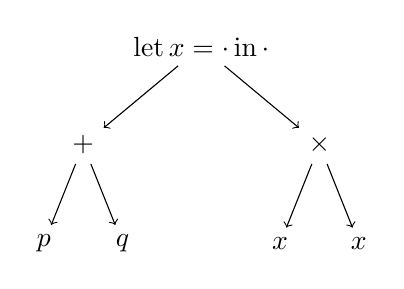
\begin{tikzpicture}
\node at (0, 2.5) (let) {$\mathrm{let}\,x=\cdot\,\mathrm{in}\,\cdot$};
\node at (-1.5, 1.25) (plus) {$+$};
\node at (-2, 0) (a) {$p$};
\node at (-1, 0) (b) {$q$};
\draw[->] (let) -- (plus);
\draw[->] (plus) -- (a);
\draw[->] (plus) -- (b);
\node at (1.5, 1.25) (times) {$\times$};
\node at (1, 0) (x1) {$x$};
\node at (2, 0) (x2) {$x$};
\draw[->] (let) -- (times);
\draw[->] (times) -- (x1);
\draw[->] (times) -- (x2);  
\end{tikzpicture}
  \caption{Abstract syntax tree}
\end{subfigure}%
\begin{subfigure}{.4\textwidth}
  \centering
\begin{tikzpicture}
\node at (0, 2.5) (times) {$\times$};
\node at (0, 1.25) (plus) {$+$};
\node at (-1, 0) (a) {$p$};
\node at ( 1, 0) (b) {$q$};
\draw[->] (times) to [out=240,in=120] (plus);
\draw[->] (times) to [out=300,in=60] (plus);
\draw[->] (plus) -- (a);
\draw[->] (plus) -- (b);
\end{tikzpicture}
  \caption{Term graph (with the let-binding inlined)}
\end{subfigure}
\caption{Comparing representations of \texttt{let x = p + q in x * x}}
\label{fig:term-repr}
\end{figure}

% dataflow computation

\subsection{Optimisations} \label{general-optimisations}

We briefly introduce typical compiler optimisations that are particularly important in this project.

Firstly, we summarise \textbf{common subexpression elimination} (CSE): whenever a program contains multiple computations of a pure expression $e$, we may instead introduce a variable $x$ defined to be $e$ and replace all existing occurrences of $e$ with $x$. 
% Simple solutions include considering sets of subterms for each subterm and dominator trees. 
In the scope of this work, we consider a special case of CSE -- transformation of a term graph into an abstract syntax tree by insertion of let-bindings.

An important optimisation for a calculus with array comprehensions is flattening loops, where nesting them is unnecessary. When a subexpression does not depend on the state of the loop it is placed in, it may be computed before the loop starts. This is termed \textbf{loop-invariant code motion}.
% It can be performed via dataflow analyses.

\section{Requirements analysis}
\label{requirements-analysis}

As outlined in the Introduction and the Proposal, the project contains the following core deliverables:
\begin{itemize}
    \item \textbf{Formalisation} of a pointful array calculus, characterising what is expressible in the DSL.
    \item \textbf{Front-end embedding} of the DSL in Python, producing programs in the introduced calculus.
    \item \textbf{Execution back-end} for running programs efficiently by targeting existing array frameworks.
\end{itemize}
There were many possible variations on any of these points, so best judgements were made to fulfil the success criteria. A deep embedding was chosen for the DSL, as it is an elegant approach that easily lends itself to metaprogramming in the host language. 
% A major extension was the introduction of user-defined types in a way compatible with the DSL. 
The calculus was originally inspired by Dex \cite{paszke2021getting}, with extensions influenced by research of \textcite{shaikhha2019efficient} on $\tilde F$. 

Since the paradigm does not possess particularly complex runtime features, a basic interpreter is easy to write. However, the goal of execution with the largest Python array programming library -- NumPy -- was prescribed, so the scope of the array calculus had to be adapted over time to the capabilities of the compilation scheme. 
% The execution method was intended to be generalisable to other array frameworks.
% No middle-end compiler phases were identified as a core deliverable, but they did form important extensions, including various compiler optimisations and program transformations.

\subsection{Methodology}

Owing to the modularity of the project and relatively orthogonal extensions, the \textit{spiral model} of development was adopted. After the initial milestones for each of the core deliverables (calculus, front-end, back-end), further ones focused on extensions. Priority was assigned based on impact on success criteria and practical usage, as well as efficiency of further work. Risk assessment relied on the existence of implementations or descriptions of a feature in the literature. Debug tooling for inspecting intermediate outputs is useful for debugging (particularly for a compiler), and as such it was also given priority.

\subsection{Review of array programs}
\label{suite-review}

Array programs vary significantly depending on the domain. One of these differences is in what language features are necessary to express them. For instance, deep learning programs rarely feature control flow, while differential equation solvers might perform iterated stencil computations. Even though application in deep learning is the original motivation, developing a more general calculus was preferable.

Due to my limited past experience with array programming applications, I conducted a comprehensive review of array programs. This assessment was conducted on 29 cases in the Futhark benchmark suite \cite{The_Futhark_Hackers_futhark-benchmarks}, with programs classified based on the language features they included.

An example conclusion from this review was the addition of a general loop primitive (fold). It allows expressing more of the reviewed programs, which the original calculus could not (it only possessed a summation). 
Furthermore, a majority of the benchmark suite in the Evaluation is based on these cases. 

\subsection{Choice of language and tools}

Python was chosen as the main language, as it is the host language for the DSL, and itself has a robust array programming ecosystem. 
In particular, NumPy's first-class interface is in Python. 
Hence, the front-end and runtime were both fixed to Python. 
Only the middle/back-end could be moved to another language -- and one with a robust Python cross-language interface. A notable example of such a language is Rust. However, attempts at an early prototype showed a trade-off due to its restrictive type system. Though it would have ensured better performance and reliability, my inexperience slowed down development. C++ is another Python-friendly alternative, but lacks language features useful for a compiler. Lastly, I considered OCaml, which is good for implementing compilers, but problematic with Python. 

As Python is not the best choice for writing a compiler, a modern Python version was used to take advantage of structural pattern matching (added in version \texttt{3.10}) and new gradual typing features. They significantly improved the code quality and programming experience. 

I chose a suite of tools standard to Python. All software applied was under a permissive open-source license, or permitted educational use.

\subsection{Version control and testing}

The main version control system applied for the project was Git. The repository was actively backed up to GitHub. All writing was done on-line in an Overleaf project synced to GitHub. I always held artefact copies on a local device. This was deemed sufficient due to high reliability standards of these services. 

Python's \texttt{pytest} testing framework was applied, which is a standard choice that I was familiar with.
Most of the code was statically typed with Python's type annotation facilities, as verified by \texttt{mypy}. It was run in addition to a linter (\texttt{ruff}) and autoformatters (\texttt{black}, \texttt{isort}, \texttt{pyupgrade}). All of the tools were run via \textit{pre-commit hooks}, ensuring a clean state of the repository at all times.

% TODO?
% \subsection{Licences}

% \textcolor{purple}{\textit{All software applied was open-source and permitted educational use: Python, NumPy, PyCharm, pytest, pre-commit hook stuff (mypy, black, ...), ...}}
% \todothis

\section{Starting point}
\label{starting-point}

Prior to starting the project, I had a solid amount of experience in Python and NumPy -- in particular through the \textit{Scientific Computing} course. I had not designed or implemented a programming language before. I had done a fair amount of reading of primary sources on array languages to establish the feasibility of the project. Material learnt in \textit{Semantics of Programming Languages} and \textit{Compiler Construction} was useful throughout the course of the project.

No implementation code was written prior to Michaelmas 2024, though I experimented with some of the elements of the project. No existing codebases were used as a basis. 
% \textit{Types}, \textit{Denotational Semantics}, and \textit{Optimising Compilers}
